% This file was converted to LaTeX by Writer2LaTeX ver. 1.0.2
% see http://writer2latex.sourceforge.net for more info
\documentclass[a4paper,12pt,twoside]{article}
\usepackage{geometry}
\geometry{a4paper,left=35mm,right=25mm, top=25mm, bottom=20mm}
\usepackage[utf8]{inputenc}
\usepackage[T1]{fontenc}
\usepackage[english]{babel}
\usepackage[pdftex]{graphicx}
\pagestyle{headings}
\usepackage{caption}[2008/08/24]
%\renewcommand{\captionfont}{\small \it}
%\renewcommand{\figurename}{Abb.}
\addto\captionsngerman{\renewcommand\figurename{Abb.}}
\addto\captionsenglish{\renewcommand\figurename{Fig.}}
\renewcommand{\floatpagefraction}{.8}
%\usepackage{url}
\usepackage{hyperref}

%\addto{\captionsngerman}{%
%    \renewcommand*{\listfigurename}{Abb.}}
%\KOMAoptions{DIV=last}
\setlength{\emergencystretch}{1em}

%Obsolete
%\newcounter{Abb}
%\renewcommand\theAbb{\arabic{Abb}}

\title{efaLive}
\author{Kay Hannay}
\date{2014-01-16}
\begin{document}
\pagenumbering{roman}
%\clearpage\setcounter{page}{1}

\begin{titlepage}
    \vspace*{1cm}
    \begin{center}
        \begin{figure}
            \centering
            
\includegraphics[width=9.745cm,height=7.308cm]{efaLiveen-img/efaLiveen-img1.png}
        \end{figure}
        \Huge
        \textbf{efaLive} \\[0.1cm]
        \LARGE
        Anleitung \\[5cm]
    \end{center}
    \normalsize
    \textbf{Datum:} 16.01.2014 \\
    \textbf{Version:} 1.5 \\
    \textbf{efaLive:} 2.2-2.1.0\_00-x86 \\
    \textbf{Kay Hannay} <klinux@hannay.de> \\
\end{titlepage}

%\clearpage\setcounter{page}{1}
%\bigskip

%\setcounter{tocdepth}{10}
%\renewcommand\contentsname{Inhaltsverzeichnis}
\tableofcontents
%\section{}
\clearpage\setcounter{page}{1}
\pagenumbering{arabic}
\section{Introduction}
This manual describes how to use the efaLive-CD and what you can do with
it.

A live-CD is a bootable CD for your computer. The whole system runs from
the CD and does not touch the hard disc. Thus, such a CD is a good tool
for demos of software, installations or to repair the software on a PC.

Another characteristic of a live-CD is, that all changes that were done
at runtime get lost when the PC is stopped. This is, because the hard
drive does not get modified and the CD is not writable. One solution
for this disadvantage is to use an USB stick. We will come back to this
later.

This CD is based on the Debian GNU/Linux \cite{DEB1} operating system.
Since Linux is open source software, you do not have to pay any license
fees to use it. Without this, it would not be possible to provide this
live-CD. This would not be possible using Microsoft Windows for legal
reasons. The same applies to efa \cite{EFA1}, which is the reason for
this CD. efa is open source software as well.

\bigskip
\textbf{ATTENTION:} Even though this CD does not touch the hard drive of your PC
it can not be guaranteed that the Live-CD anyhow influences the
behavior of the PC. I have to point out that you use the CD on your own
risk. I am not responsible for any damage on your hard- or software.
\bigskip

\section{efaLive-CD}
\label{sct:efalivecd}
\subsection{Hardware requirements}
\label{sct:live_hardware}
Here you can see the hardware requirements for the live-CD. The values
are minimal requirements.

\begin{itemize}
    \item Intel Pentium III Processor at 600MHz
    \item 128 MB memory
    \item CD-ROM drive or USB connector
    \item Monitor with a resolution of 1024x768 pixels
    \item optional an USB connector for backups
\end{itemize}

\subsection{How to create the efaLive-CD}
\label{sct:create_cd}
You can download an efaLive ISO image from the Internet \cite{EFA4}.
Almost all CD recording software provides a functionality to burn such
ISO CD images on a CD. Check the documentation of the software for more
information.

As an alternative you can copy efaLive to a USB stick.


\subsection{Or use an USB stick}
\label{sct:usb_stick}
Since efaLive version 1.2 it is possible to copy it on an USB stick. The
PC has to be able to boot from USB devices to use this method.
Especially older PCs often do not have this functionality.

On Linux you can copy the ISO image using the command \texttt{dd
if={\textless}EFA LIVE ISO{\textgreater} of=/dev/sdb}
(provided /dev/sdb is the USB stick). Attention: it is possible to
delete important data if you do not choose the correct device for the
\texttt{of=} parameter!

On Windows you can use the Win32 Disk Imager \cite{IMG1}.This program by
default works for \texttt{.img} files only. So you
have to rename the file or change the field „file name“ to
\texttt{*.iso}.

Besides that there is no difference compared to a CD.


\subsection{How to run the efaLive-CD}
\label{sct:live_run}
Starting the live-CD is quite easy:

\begin{enumerate}
    \item Put the CD into the CD-ROM drive or plug in the USB stick
    \item (Re-) start the computer
    \item Select efaLive (English) on the selection screen
(Fig.~\ref{fig:syslinux}) and press {\textless}Enter{\textgreater}
\end{enumerate}

\begin{figure}
    \centering
    \fbox{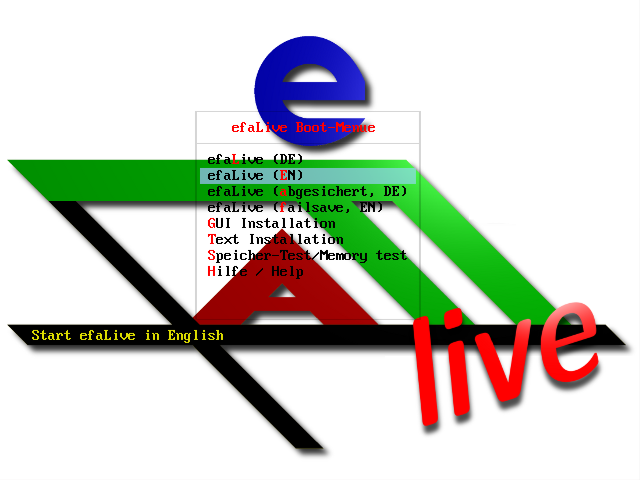
\includegraphics[width=10cm]{efaLiveen-img/efaLiveen-img2.png}}
    \caption{Selection screen boot loader (Syslinux)}
    \label{fig:syslinux}
\end{figure}

efa will be started automatically with its boat house view when you run
the live-CD. You can find more information about the usage of efa in
its documentation \cite{EFA2}.

You should see a screen like in Fig.~\ref{fig:efalivesetup_live} after a while.
Here you can choose the version of efa, that you would like to use. I
recommend version 2, since version 1 is not maintained any more and efa
2 has many benefits compared to version 1. Click on „Ok“ after your
selection.

The efaLive Setup window can always be opened by pressing
\texttt{{\textless}Strg{\textgreater}+{\textless}F12{\textgreater}}. So you can
change these settings at any time. For some settings it is necessary to
restart the PC to take effect. You have to pass the password of the efa
user before the window is opened.

\begin{figure}
    \centering
    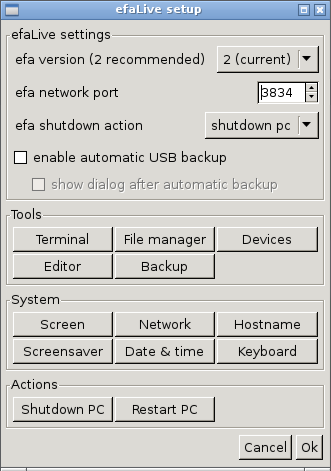
\includegraphics[width=8cm]{efaLiveen-img/efaLiveen-img3.png}
    \caption{efaLive Setup}
    \label{fig:efalivesetup_live}
\end{figure}

The default password for the root user is „livecd“, the one for the efa
user is „efalive“.

An English keyboard layout is used, if you have started the live-CD in
the English mode.


\subsection{Persist data in live mode}
\label{sct:live_persist}
To persist the changes during a live session you can use an USB stick.
You have to uncompress the file persistence.zip from the snapshot
directory of the CD to the root folder of any USB stick so that there
is a "persistence" file. Plug in this stick
into the PC before you start it from the live-CD. The stick should be
recognized by the PC during the boot phase. It will be used for
snapshots of the home directory of the efa user. This means that the
content from the persistence file is copied to the home directory at
startup and vice versa at shutdown. The home directory contains
configuration data and user data of efa.

Since the copy process runs at boot and shutdown only, you should not
remove the USB stick before the PC was shut down.


\section{Installation}
\label{sct:installation}
\subsection{Hardware requirements}
\label{sct:inst_hardware}
These are minimum requirements.

\begin{itemize}
    \item Intel Pentium III processor with 600MHz
    \item 128 MB memory
    \item 2 GB hard disc
    \item CD-ROM drive or USB connector (for installation)
    \item Monitor with a resolution of 1024x768 pixel
    \item optional an USB slot for backups
\end{itemize}

The memory might be even less than stated above, but you can not run the
graphical installer in that case. The installation in text mode is no
rocket science, but it is not described in this document.

You should think about hardware components that are really required for
the usage in the boat house, before you start the installation. Read
more about this in chapter \ref{sct:periphery}.


\subsection{Installation steps}
\label{sct:inst_steps}

\begin{minipage}{\linewidth}
    \centering
    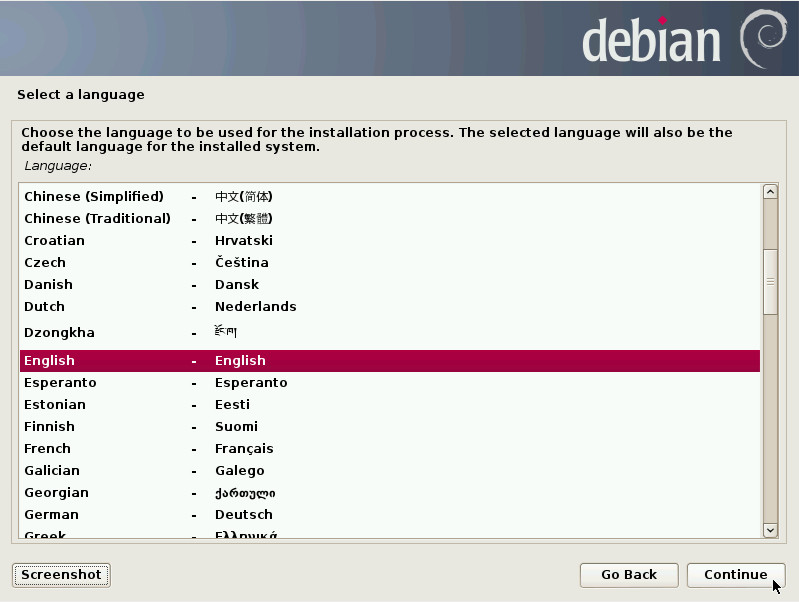
\includegraphics[width=10cm]{efaLiveen-img/efaLiveen-img4.png}
    \captionof{figure}{Choose the language}
    \label{fig:inst_language}
\end{minipage}
\bigskip

In this document I only can cover very common aspects of the
installation. Thus I assume that you use a standard desktop PC with a
hard drive, a CD-ROM drive and optional one wired network card. Further
on I assume that the whole hard drive gets used for the installation so
that all data get deleted. For more information regarding the
installation of the Debian GNU/Linux system check \cite{DEB2}.

\textbf{ATTENTION:} Strictly following this installation instructions, the whole
hard drive of the PC will be erased! All data on the hard drive will be
lost! It is possible to influence this behavior, but this is not part
of this document.

In the first step you have to choose the language you want to use for
the installation and the system. After a click on
"Continue" you have to choose the country
and the keyboard layout.


\subsubsection{Computer without network card}
\label{sct:inst_no_net}

\begin{minipage}{\linewidth}
  \centering
  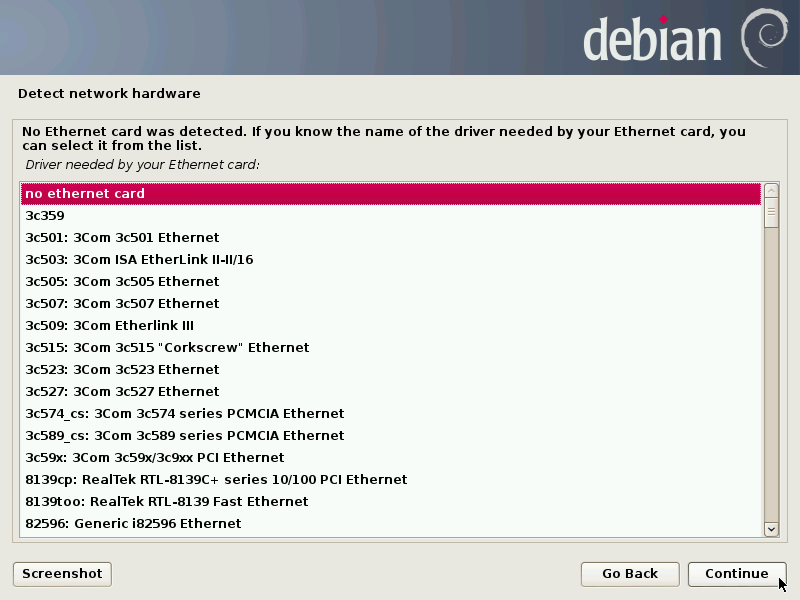
\includegraphics[width=10cm]{efaLiveen-img/efaLiveen-img5.png}
  \captionof{figure}{Auswahl Netzwerkkarte}
  \label{fig:inst_netzwerkkarte}
\end{minipage}
\bigskip

Most modern computers have a network card. Thus the installation program
is very eager to find such a card. Choose "no Ethernet card" here.

The next screen contains a warning that no network card was found. You can
just confirm it. The next section can be skipped.

\bigskip
\begin{minipage}{\linewidth}
  \centering
  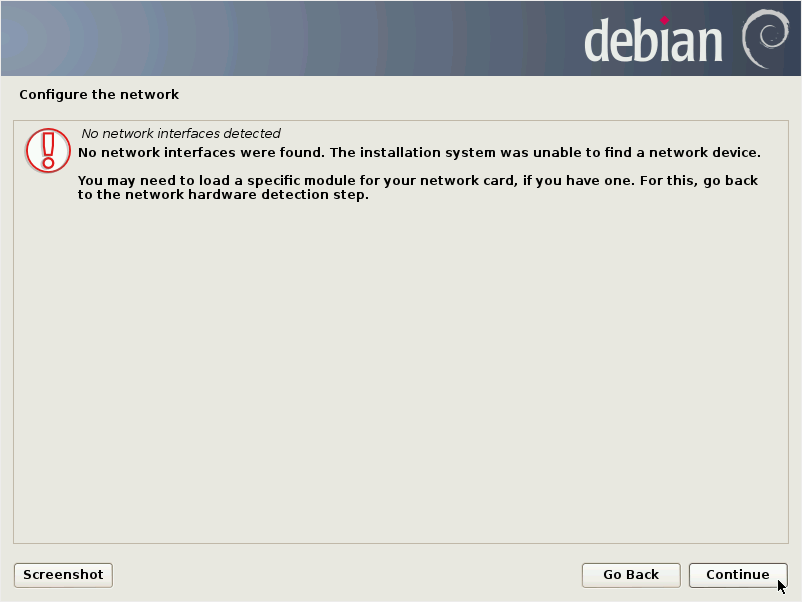
\includegraphics[width=10cm]{efaLiveen-img/efaLiveen-img6.png}
  \captionof{figure}{Confirmation of network card}
  \label{fig:inst_conf_net}
\end{minipage}


\subsubsection{Computer with network card}
\label{sct:inst_with_net}
Usually there is a DHCP server in a network with DSL or any similar
Internet connection. It automatically configures the network card with
the correct settings for the network. Normally a DHCP server runs on
the Router. In case that the automatic configuration via DHCP does not
work, you will see a note like in \ref{fig:dhcp_error}. Otherwise, the
network will be configured automatically and you can continue with the
hard drive setup.

\bigskip
\begin{minipage}{\linewidth}
    \centering
    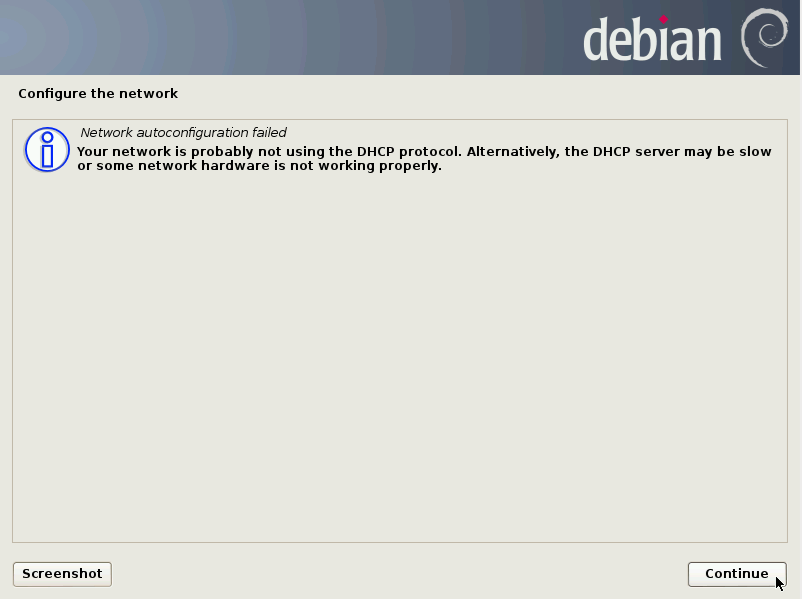
\includegraphics[width=10cm]{efaLiveen-img/efaLiveen-img7.png}
    \captionof{figure}{DHCP configuration failed}
    \label{fig:dhcp_error}
\end{minipage}
\bigskip

You can confirm this screen. In the next step you have to choose, how to
configure the network. Did the DHCP configuration fail, even there is a
DHCP server in your network, you have to check what's
wrong and choose "retry network autoconfiguration".

Another choice is to not configure the network. I think, this is not
very useful, because in this case you should better disable or remove
the network card (see chapter \ref{sct:periphery}).

\bigskip
\begin{minipage}{\linewidth}
    \centering
    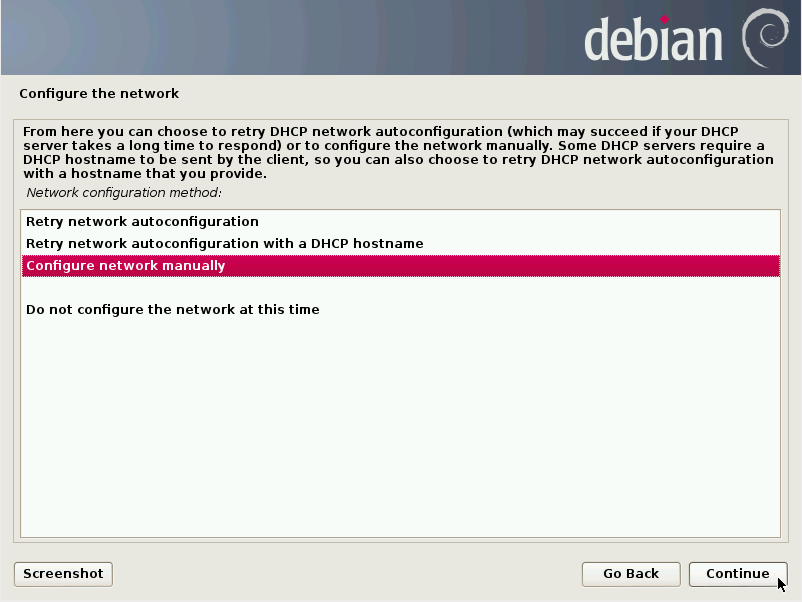
\includegraphics[width=10cm]{efaLiveen-img/efaLiveen-img8.png}
    \captionof{figure}{Manual configuration of the network}
    \label{fig:network_manual}
\end{minipage}
\bigskip

Most probably you want to configure the network manually now. So choose
the corresponding entry in the list. In the following steps you get
asked for the IP address for the PC, the network mask, the gateway and
the name server (DNS). Please take care here. If you choose wrong
settings, you can disturb the whole network!


\subsubsection{Configure time zone}
\label{sct:inst_timezone}

Depending on the country you have selected before, a dialog to choose
your time zone may be shown.

\bigskip
\begin{minipage}{\linewidth}
    \centering
    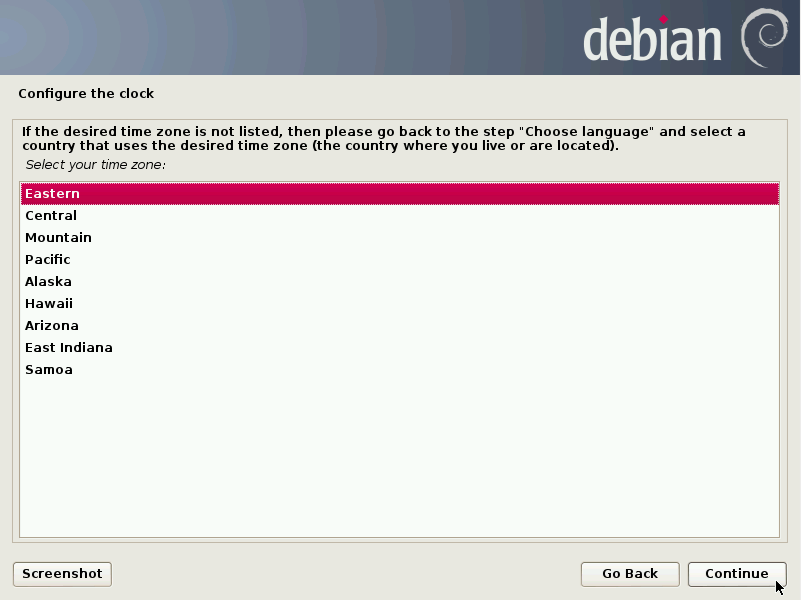
\includegraphics[width=10cm]{efaLiveen-img/efaLiveen-img9.png}
    \captionof{figure}{Time zone settings}
    \label{fig:inst_timezone}
\end{minipage}


\subsubsection{Hard drive setup}
\label{sct:inst_harddrive}

\begin{minipage}{\linewidth}
    \centering
    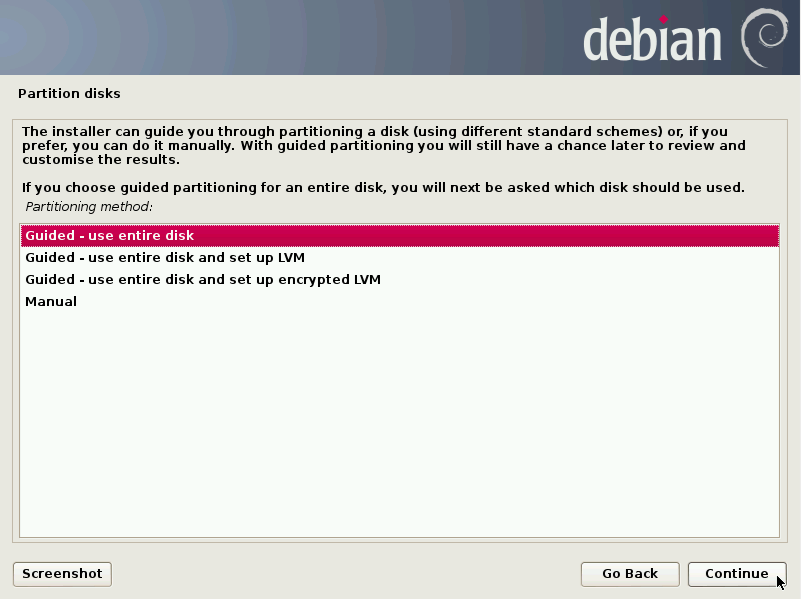
\includegraphics[width=10cm]{efaLiveen-img/efaLiveen-img10.png}
    \captionof{figure}{Partitioning}
    \label{fig:partitioning}
\end{minipage}
\bigskip

Now you have to partition the hard drive. This means that the hard drive
is divided into proper sections for the usage with efaLive. I assume
that the whole hard drive shall be used here. This means that all data
on the hard drive will be deleted!

You can influence this behavior by choosing
"Manual", but you should know what you are
doing in this case.

\bigskip
\begin{minipage}{\linewidth}
    \centering
    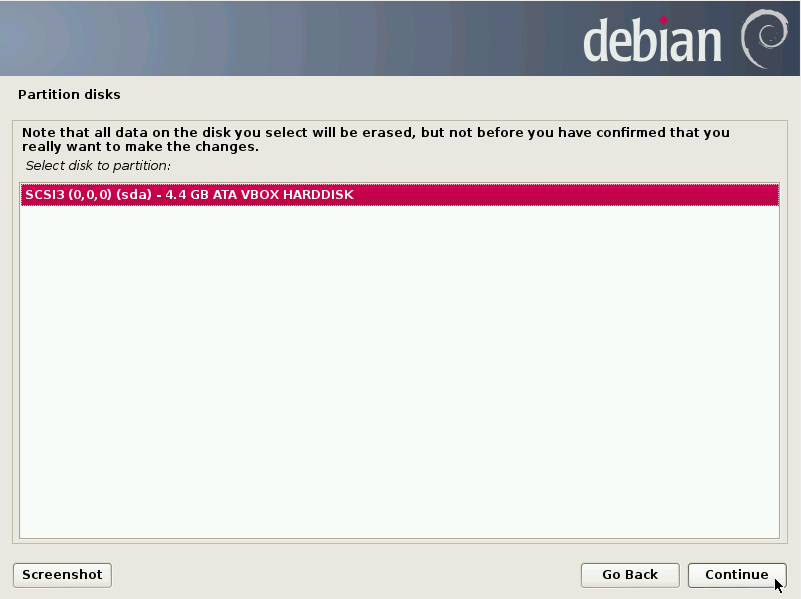
\includegraphics[width=10cm]{efaLiveen-img/efaLiveen-img11.png}
    \captionof{figure}{Auswahl Festplatte}
    \label{fig:auswahl_festplatte}
\end{minipage}
\bigskip

Here you have to choose the hard drive for the installation. In this
example there is only one.

\bigskip
\begin{minipage}{\linewidth}
    \centering
    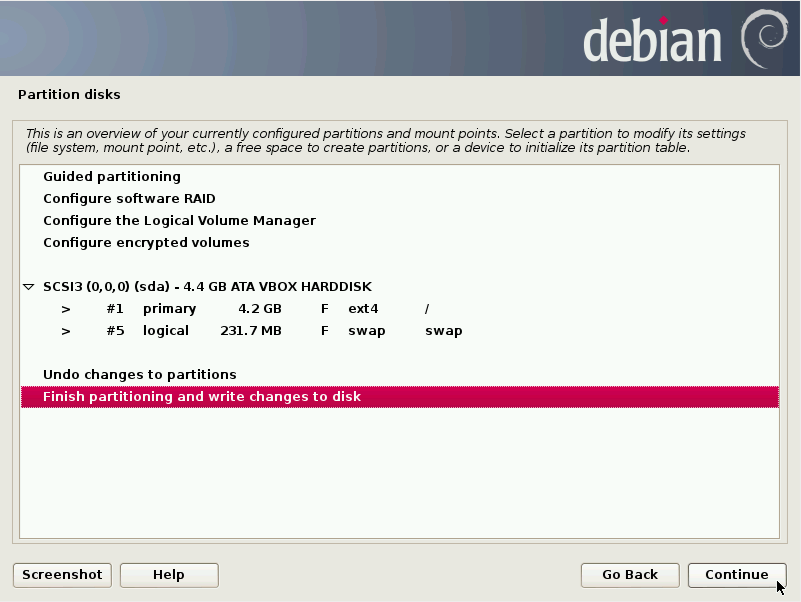
\includegraphics[width=10cm]{efaLiveen-img/efaLiveen-img12.png}
    \captionof{figure}{Confirm partitioning}
    \label{fig:conf_partitioning}
\end{minipage}
\bigskip

On the next screen you can see, how the hard drive will be partitioned.
Choose "Finish partitioning and write changes to disk" to continue.

\bigskip
\begin{minipage}{\linewidth}
    \centering
    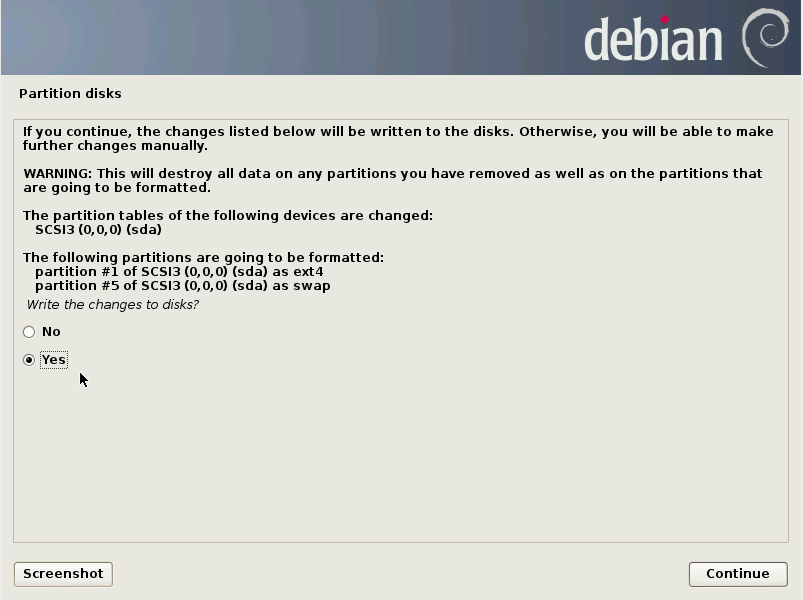
\includegraphics[width=10cm]{efaLiveen-img/efaLiveen-img13.png}
    \captionof{figure}{Security question before writing to hdd}
    \label{fig:conf_write_hdd}
\end{minipage}
\bigskip

You see another warning now. All data on the hard drive will be deleted,
if you choose "Yes" here.


\subsubsection{Package management}
\label{sct:package_management}

\bigskip
\begin{minipage}{\linewidth}
    \centering
    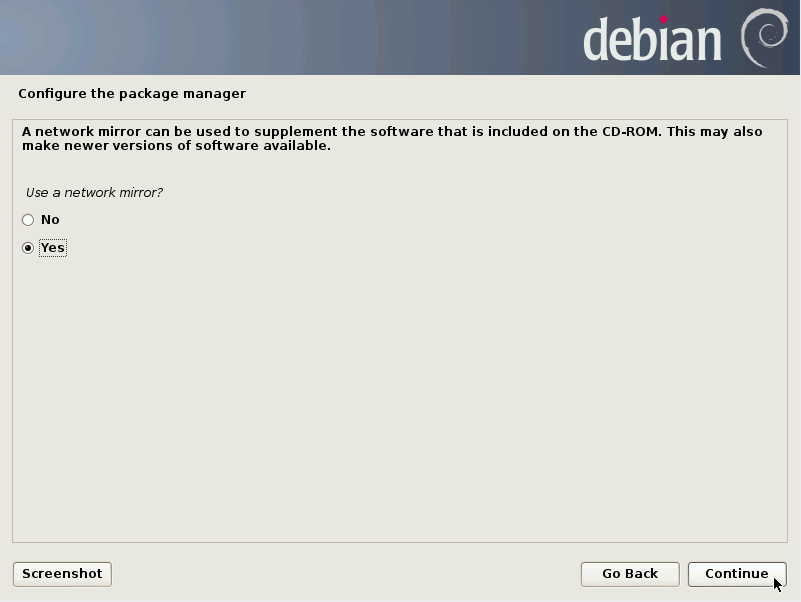
\includegraphics[width=10cm]{efaLiveen-img/efaLiveen-img14.png}
    \captionof{figure}{Use a mirror server?}
    \label{fig:use_mirror}
\end{minipage}
\bigskip

The Linux system which efaLive is based on can be updated over the
Internet. To get the best download performance and to disburden the
main software package servers, you should choose a proper mirror
server. It should be close to your location to get the best results.

Choose "No" here, in case your computer has
no Internet connection.

\bigskip
\begin{minipage}{\linewidth}
    \centering
    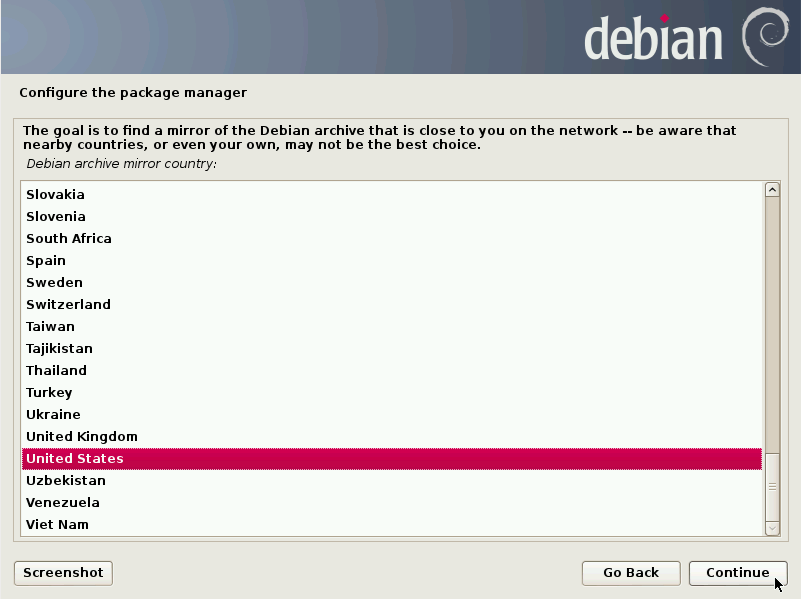
\includegraphics[width=10cm]{efaLiveen-img/efaLiveen-img15.png}
    \captionof{figure}{Region for mirror server}
    \label{fig:mirror_region}
\end{minipage}
\bigskip

If you decided to use a mirror server, you first have to select the
region where you are located. Then you get a list of mirror servers
that are based in that region. Choose one of them that is close to you.

\bigskip
\begin{minipage}{\linewidth}
    \centering
    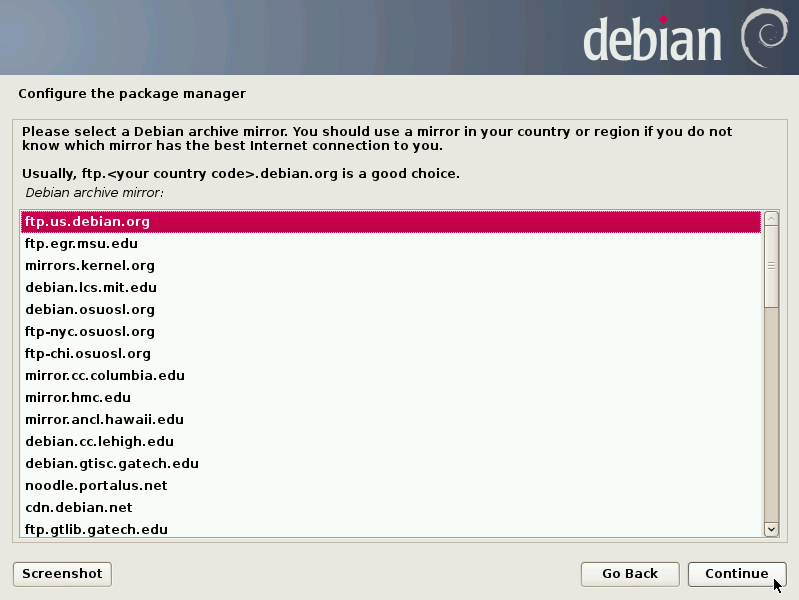
\includegraphics[width=10cm]{efaLiveen-img/efaLiveen-img16.png}
    \captionof{figure}{Choose a mirror server}
    \label{fig:choose_mirror}
\end{minipage}
\bigskip

\begin{minipage}{\linewidth}
    \centering
    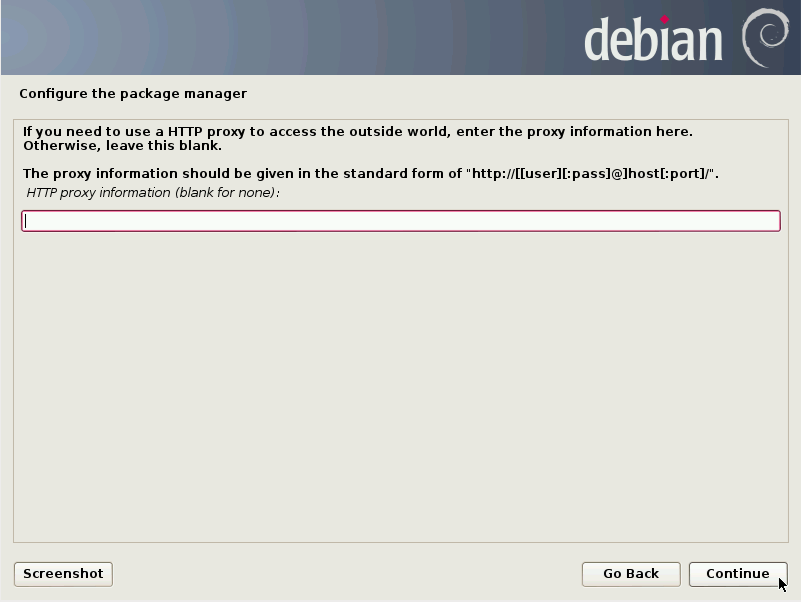
\includegraphics[width=10cm]{efaLiveen-img/efaLiveen-img17.png}
    \captionof{figure}{Use proxy server}
    \label{fig:select_proxy}
\end{minipage}
\bigskip

Now you can configure a Proxy server. In most cases you can leave this
field blank and continue.


\subsubsection{Boot loader}
\label{sct:boot_loader}

\begin{minipage}{\linewidth}
    \centering
    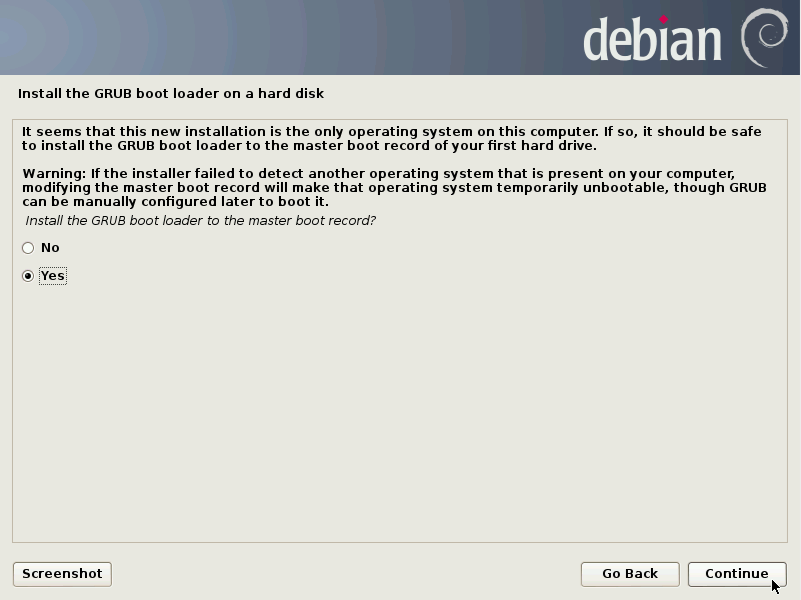
\includegraphics[width=10cm]{efaLiveen-img/efaLiveen-img18.png}
    \captionof{figure}{Install boot loader Grub}
    \label{fig:inst_grub}
\end{minipage}
\bigskip

Now you're almost done. The last question asks you,
where to install the boot loader. It is not important what a boot
loader is, at the moment. Normally you should choose
"Yes" here to install it into the master
boot record.

\bigskip
\begin{minipage}{\linewidth}
    \centering
    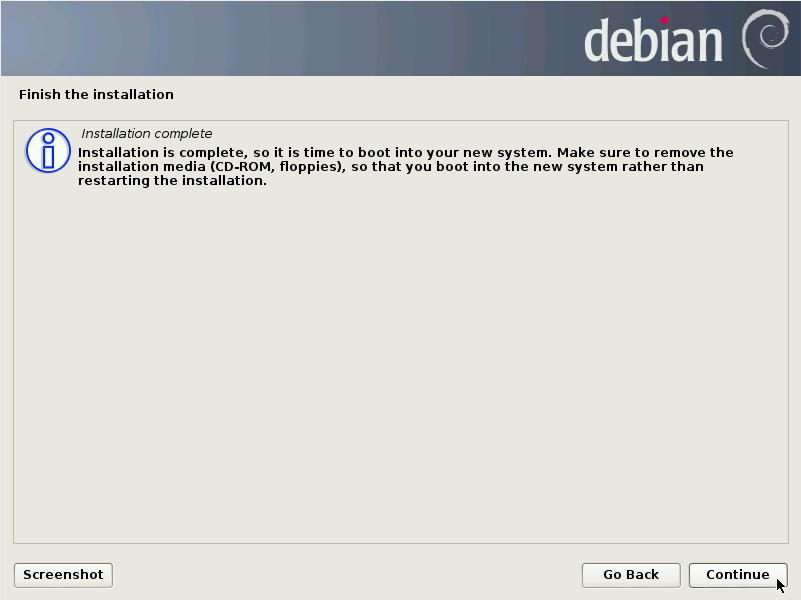
\includegraphics[width=10cm]{efaLiveen-img/efaLiveen-img19.png}
    \captionof{figure}{Finish}
    \label{fig:finish}
\end{minipage}
\bigskip

That's it! The installation is finished. After clicking
on "Continue", the computer will be
restarted. Remove the CD-ROM or the USB Stick now, so that the PC does
not boot from it again.

When you start the computer from hard disc now, you will not see the
boot loader like in \ref{fig:syslinux}. The boot loader that was just
installed prints a short text only. You can press
\texttt{{\textless}ESC{\textgreater}} here if you want to enter the menu of the
boot loader. To edit one of the menu entries, you have to authenticate.
The default user is "root" and the password "livecd".

Without pressing a key, the system boots efaLive. You can hide the image
that is shown during startup to watch the boot messages by pressing
\texttt{{\textless}ESC{\textgreater}}.

Now I suggest you to read chapter \ref{sct:system_secure} to
secure your fresh efaLive installation.

\bigskip
Information for the usage of efa can be found on \cite{EFA2}.

\bigskip
Have fun with efaLive!


\section{Administration of the system}
\label{sct:administration}
\subsection{Local access}
\label{sct:local_access}
You can use efaLive-Setup or a console for
administrative tasks. Some of these tasks can be performed as user
"efa". For other tasks you need the
privileges of the "root" user, who is the
administrator of a Linux system. With these privileges you can do
everything with the system, even erase the whole hard disk. So please
be careful when you work as user "root".

In the following sections you can read here and there that you should
log in as user "efa" or
"root". This means that you should change
to a text console (chapter \ref{sct:text_console}) or use
the console of efaLive-Setup (chapter \ref{sct:toolbox})
using the "Terminal" button of the tool
box.

After finishing your administrative tasks, you should leave the console
by using the "exit" command. The console
from the efaLive-Setup can also be closed by clicking in the X of the
console window. Please don't forget this step,
otherwise any user can run commands in that console. To be sure, you
can use \texttt{{\textless}Alt{\textgreater}+{\textless}Tab{\textgreater}} to
check if there are any other windows than efa open.


\subsubsection{Tool box}
\label{sct:toolbox}
The "tool box" from efaLive-Setup is the preferred way to start a
console. After starting it, you are logged in as user
"efa". You have to provide the
corresponding password when you start efaLive-Setup. To get
"root" privileges you have to type
\texttt{su -}, followed by the
"root" password.

Use \texttt{{\textless}Strg{\textgreater}+{\textless}F12{\textgreater}} to start
efaLive-Setup from within efa. For more information on efaLive-Setup
see chapter \ref{sct:efalivesetup}.

\subsubsection{Text console}
\label{sct:text_console}
On Linux systems you can switch
between the graphical user interface and text consoles. This is done by
key combinations from
\texttt{{\textless}Ctrl{\textgreater}+{\textless}Alt{\textgreater}+{\textless}F1{\textgreater}} to\\
\texttt{{\textless}Ctrl{\textgreater}+{\textless}Alt{\textgreater}+{\textless}F7{\textgreater}}.
Normally you have six text consoles and one graphical interface. It
depends on the installation where the graphical interface is located.

On a text console you just see a text prompt that asks for a user name.
So to log in as user "root" you have to
pass "root" as the user name at
"login:", confirm with
\texttt{{\textless}Enter{\textgreater}} and then provide the password for the
"root" user. Please note that your key
presses are not confirmed by any output on the screen when you type in
the password.


\subsection{Remote access}
\label{sct:remote_access}
efaLive is equipped with a SSH server. Via SSH you can log in into a
computer via network. On Linux based PCs, SSH is normally
pre-installed. For Windows you can use for example Putty \cite{PUT1}.

On Linux you can use a command like \texttt{ssh
efa@efalive.efa.local} to connect to the efaLive system.
You get a text console like mentioned in chapter \ref{sct:text_console}. In a small
network you might have to use the IP address of the efaLive system
after the \texttt{@} character instead of the
name.

For security reasons it is not allowed to log in as user
"root" directly. To work as
"root" user, you have to log in as
"efa" and use the command \texttt{su -} like in chapter \ref{sct:toolbox}.

If you want to access the efaLive system from the Internet and the
system is not directly connected to the Internet, you have to enable a
port forwarding on the router. There you can use a port, like for
example 1234, and forward it to the network name or IP address of the
efaLive system to port 22. Do not use port 22 as the forwarded port on
the router. This is the default port for SSH and there are many attack
attempts from the Internet on this port.

It is very important to choose a strong password for the
"efa" user if the system is accessible from
the Internet! It should be long, contain capitalized and
non-capitalized characters, numbers and special characters.


\subsection{Data backup}
\label{sct:data_backup}
\subsubsection{Backup}
\label{sct:backup}
You can configure efaLive in a way
that it automatically creates a backup on a USB stick when the stick is
plugged in.

On success you will probably hear three short beep tones. In case of an
error, you will hear 5 long beep tones. In this case you can leave the
stick in the PC and mount it from the tool box. Log in as user
"efa" and create a manual backup by running
the command \texttt{efalive-backup /media/{\textless}MOUNT
POINT{\textgreater}}. The place holder
"{\textless}MOUNT POINT{\textgreater}" has
to be replaced by the mount point of the USB stick. Now you can
probably see error messages.

In case the backup was successful, you can unplug the USB stick. It is
unmounted automatically after the backup.

For PCs that don't have a speaker or for other reasons
don't play the tones, you can configure to show a
dialog instead. This is done in efaLive-Setup (chapter \ref{sct:efalivesetup}).

You now should have a directory called
\texttt{efaLive\_backup\_YYYYMMDD\_HHMMSS} on your
USB stick. \texttt{YYYYMMDD} stand or the actual
date and \texttt{HHMMSS} stand for the actual
time. In that directory you find two ZIP files,
\texttt{efa\_backup\_YYYYMMDD\_HHMMSS.zip} and
\texttt{efaLive\_backup\_YYYYMMDD\_HHMMSS.zip}.
The first one contains the efa backup, the second one the configuration
backup of efaLive.

The efaLive backup only contains some settings from efaLive-Setup. Other
modifications of the system must be backup-ed separately. This is a
compromise to store as many settings as possible, but
don't let the backup grow too much.

Another way to create a backup is to use the tool box, see chapter \ref{sct:toolbox}. Or
you can use the command line and run
\texttt{efalive-backup} as mentioned before.

Note efa 1: The backup for efa 1 contains one file only. Its name is\\
 \texttt{efaLive\_backup\_YYYYMMDD\_HHMMSS.zip}.


\subsubsection{Restore}
\label{sct:restore}
The most simple way to restore a backup is the devices dialog (chapter
\ref{sct:dialog_devices}). Here you can restore the backup directly from an USB stick.
Another solution is to use the backup dialog (chapter \ref{sct:dialog_backup}). The third
way is to use the command line. Log in as user
"efa" and run the command
\texttt{efalive-restore {\textless}BACKUP{\textgreater}}. Replace
\texttt{{\textless}BACKUP{\textgreater}} with the
path of one of the ZIP files in the efaLive backup directory. Please
note that both ZIP files of a complete efaLive backup have to be located in the
same directory. It is also possible to restore a efa-only or efaLive-only backup.
In this case a warning message is shown which says that there was not a complete
efaLive backup restored.

In case you did restore an efa-only backup from a non-efaLive system, you have
to create the efaLive admin user afterwards. This can be done in the admin mode
of efa under "Administrators" - "Repair Admin efaLive".

You should restart the PC after you have restored a backup so that all
settings take effect. You can use efaLive-Setup for restart.


\section{efaLive-Setup}
\label{sct:efalivesetup}
efaLive-Setup is used to configure
many things of the efaLive system. Besides that, it includes the
"tool box". Here you can find several small
tools that might be useful for administration purposes.

\begin{figure}
    \centering
    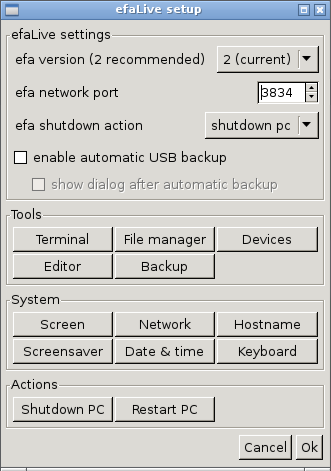
\includegraphics[width=8cm]{efaLiveen-img/efaLiveen-img20.png}
    \caption{efaLive Setup}
    \label{fig:efalivesetup}
\end{figure}

The first combo box lets you configure the version of efa you want to
use. This setting can be changed at any time. After a restart of the PC
the configured version of efa is started automatically.

The network port is relevant for efa 2 only. You only have to change it
if you have configured another port in the efa 2 settings.

With "efa shutdown action" you can configure
the action that is performed when the efa program is closed. Default is
to shutdown the PC. If this is not what you want, you can set here to
restart the PC or to restart efa.

Per default the automatic backup on USB sticks is disabled. You can
enable it here. In case you have enabled it, you can also set whether a
dialog should be shown after the backup. This is useful if you
don't have a PC speaker.

Please note that anybody who has access to an USB port of the PC can
create a backup when automatic backup is enabled. The backup might
contain sensible configuration data like passwords.


\subsection{Terminal}
\label{sct:terminal}
The terminal, or text console, can be used for many purposes that are
described in this document. After the start you are logged in as user
"efa". To get "root" access, you can use the \texttt{su -} command.


\subsection{File manager}
\label{sct:file_manager}
With this button you can start a simple file manager. You can for
example copy, move or delete files and directories, edit files and many
things more.

\subsection{Devices}
\label{sct:dialog_devices}
To mount or unmount an USB stick or
to create a backup or restore a backup from an USB stick you can use
the devices dialog.

\begin{figure}
    \centering
    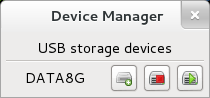
\includegraphics[width=6cm]{efaLiveen-img/efaLiveen-img21.png}
    \caption{Devices tool}
    \label{fig:dialog_devices}
\end{figure}

In the dialog you can see all USB storage devices that were found. Each
device has three buttons. The first one is to mount or unmount the
device. The second one is to create a backup on this device. And the
third one to restore a backup. Therefor a dialog is shown, where you
can select a backup file (.zip). More under \ref{sct:restore}

When you move the mouse pointer over the name of a device and leave it
there for a while, a popup is shown that holds some information for the
device. Here you can find the mount point for example.

Under "Device" you can find the device file
name which is used to access the device.


\subsection{Editor}
\label{sct:gui_editor}
Using this button you can start a
small editor called "leafpad". You can use
it for example to edit configuration files like mentioned in chapter
\ref{sct:editor}.


\subsection{Backup}
\label{sct:dialog_backup}
This tool is used to create or restore
a backup. It works similar to the devices dialog, but you can choose
the backup directory here. So after a click on
"Backup" another dialog is shown where you
have to select a target directory for the backup. Finally a small
dialog is shown to inform you whether the action was successful.

\bigskip
\begin{minipage}{\linewidth}
    \centering
    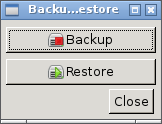
\includegraphics[width=4cm]{efaLiveen-img/efaLiveen-img22.png}
    \captionof{figure}{Backup}
    \label{fig:dialog_backp}
\end{minipage}
\bigskip

After a click on "Restore", a dialog is shown, where you can select a backup file.
More under \ref{sct:restore}.


\subsection{Logs}
\label{sct:logfiles}
This button can be used to create a ZIP file containing the most important log
files of the system. The target directory for the log file package can be selected
in a dialog.


\subsection{Screen setup}
\label{sct:screen_setup}
This tool helps you to configure the screens that are connected to your
PC.

\bigskip
\begin{minipage}{\linewidth}
    \centering
    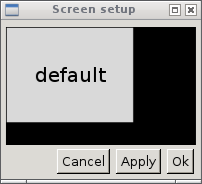
\includegraphics[width=8cm]{efaLiveen-img/efaLiveen-img23.png}
    \captionof{figure}{Screen setup tool}
    \label{fig:screen_setup}
\end{minipage}
\bigskip

Each detected screen is shown here as a gray rectangle with a name
inside. A right click on one of these rectangles opens a context menu.
Here you can en- or disable a screen, set its resolution or rotate it.
By pressing and holding the left mouse button on one of the rectangles
you can move them. This is used to position the screens relative to
each other.

A click on "Apply" activates the settings
for the current view. After a click on "Ok"
the settings are stored and applied on each start of efaLive.


\subsection{Network}
\label{sct:network}
With this button you start a tool named
"Network-Manager". You can configure almost
any kind of network connection with this tool. I will explain some
specialties here. For more information you can check the
Network-Manager documentation on \cite{NWM1}.

\bigskip
\begin{minipage}{\linewidth}
    \centering
    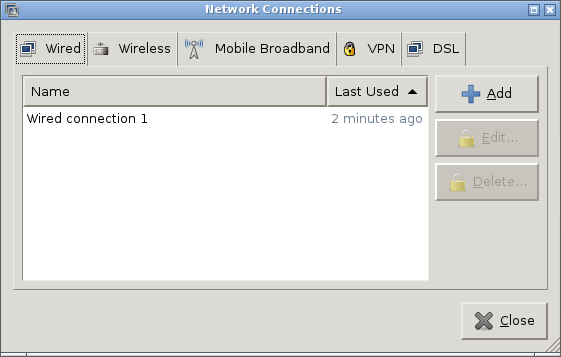
\includegraphics[width=12cm]{efaLiveen-img/efaLiveen-img24.png}
    \captionof{figure}{Network settings}
    \label{fig:dialog_network}
\end{minipage}


\subsubsection{Wifi}
\label{sct:wifi}
The tab "Wireless" is used to configure a
Wifi. After a click on "Add" you should
fill in the SSID, which is the name of the network, the type of
security, the password and select "Available to all
users". Probably you also want to enable the
"Connect automatically" option.

\begin{figure}
    \centering
    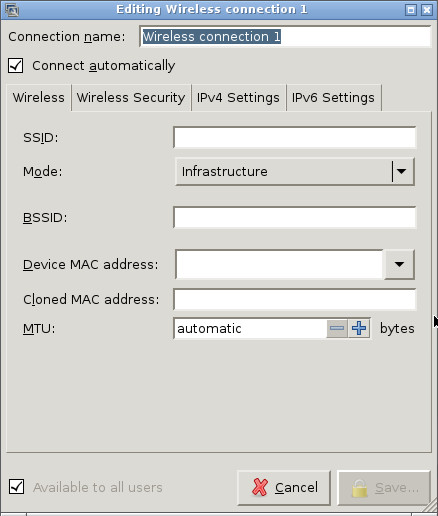
\includegraphics[width=13cm]{efaLiveen-img/efaLiveen-img25.png}
    \caption{Wifi settings}
    \label{fig:wifi}
\end{figure}


\subsubsection{Broadband}
\label{sct:broadband}
It is even possible to configure broadband connections like UMTS here.
You can start a wizard by clicking on
"Add". The wizard asks you for the provider
you use and the settings. Finally you might have to fill in the PIN for
your SIM card. The option "Connect
automatically" unfortunately does not work. But efaLive
has a function to overcome this problem. This requires that the name of
the connection is "broadband". If this is
the case, efaLive checks every 5 minutes whether there is any active
connection. If not, it tries to start the
"broadband" connection.

\bigskip
\textbf{Attention:} Using a broadband connection, depending on the type of
contract, might produce high costs! So do not use this function if you
don't have a proper contract.
\bigskip

\subsubsection{Keyboard}
\label{sct:keyboard}
Use this tool to configure your keyboard. You can change settings for
the device as well as the layout.


\subsubsection{Screen saver}
\label{sct:screen_saver}
To change the settings for the screen saver or the power saving options,
you can use this tool.


\subsubsection{Date and time}
\label{sct:date_time}
With this program you can set the date and the time of the PC. Default
is to use the "Network Time Protocol". So
the time of the PC is synchronized via Internet. This only works, if
the PC has a connection to the Internet, of course.

\begin{figure}
    \centering
    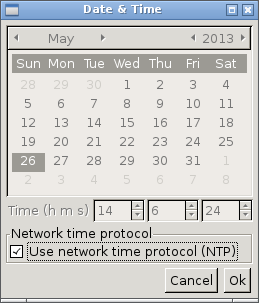
\includegraphics[width=7cm]{efaLiveen-img/efaLiveen-img26.png}
    \caption{Settings for date \& time}
    \label{fig:date_time}
\end{figure}


\subsubsection{Actions}
\label{sct:actions}
Currently you can find two buttons here. One to shut down the PC and the
other one to restart it. Both actions have to be confirmed in a small
dialog so that the PC is not stopped by accident.


\section{Software management}
\label{sct:software_management}
\subsection{Update efa}
\label{sct:update_efa}
In case you want to use a more recent version of efa, it is not required
to reinstall the whole system. You can use the built in update function
of efa.

Another way is to download the latest version from the Internet
\cite{EFA1} and copy it to an USB stick. Plug this stick into the PC
and mount it by using the tool box. Then log in as
"efa" and use the following commands:
\bigskip
\\
\texttt{cd /usr/lib/efa2
unzip -o /media/{\textless}MOUNT POINT{\textgreater}/{\textless}NAME OF
EFA FILE{\textgreater}}

\bigskip
\texttt{{\textless}MOUNT POINT{\textgreater}} is the name of the USB stick in the
\texttt{/media/} directory. \texttt{{\textless}NAME OF EFA FILE{\textgreater}} is the
name of the file that you have downloaded, for example
\texttt{efa2.zip}.

After a restart of the PC the new version should be started
automatically.

In case you use efa 1, you have to use \texttt{/usr/lib/efa} in the command
above.


\subsection{Linux software management}
\label{sct:linux_software}
To install additional software or to update already installed software,
you have basically three choices.

First, you can download and install software packages manually. Second,
you can install software from a CD. And third, you can configure
efaLive to download and install software by command. This requires an
Internet connection.

This system currently uses the "Wheezy" Debian distribution.


\subsubsection{Install software manually}
\label{sct:software_manually}
On \cite{DEB3} you can download software packages for efaLive. These
software packages have the file ending
\texttt{.deb} and can can be installed by using
\texttt{dpkg}. One problem of the manual
installation is, that many software packages have dependencies on other
packages. So if you want to install program X, it might require program
Y to be installed. All the dependencies are mentioned on the download
web page, but it is hard to know, which of the dependencies are
installed already. So I can suggest this way for very small software
packages only.

Here you can't use the instructions mentioned in \ref{sct:software_management}.
You have to use the command \texttt{dpkg -i {\textless}SOFTWARE
PACKAGE 1{\textgreater} {\textless}SOFTWARE PACKAGE 2{\textgreater}
...} as user "root" to install packages.


\subsubsection{Software from CDs}
\label{sct:software_cd}
You can download complete CD images of the Debian distribution from
\cite{DEB4}. In this case you have a huge amount of software packages
available offline. Depending on your requirements, you
don't need to download all CDs. After downloading one
or more CDs, you can use the command \texttt{apt-cdrom
add} as user "root" to
register the CDs in the system. The program asks you to insert one CD
after the other.

Use this method if your PC does not have an Internet connection.


\subsubsection{Software directly from the Internet}
\label{sct:software_internet}
With an Internet connection, this is the best way to install or update
software. In case you selected a mirror at installation time, you can
start directly. If not, you have to add this mirror server now. Use the
following commands as user "root":
\bigskip
\\
\texttt{echo "deb http://ftp.us.debian.org/debian/ wheezy main contrib \textbackslash\\
    non-free"\ {\textgreater}{\textgreater} /etc/apt/sources.list}
\\
\texttt{echo "deb-src http://ftp.us.debian.org/debian/ wheezy main contrib \textbackslash\\
    non-free"\ {\textgreater}{\textgreater} /etc/apt/sources.list}

\bigskip
After that you have to update the internal index by using the command
\texttt{aptitude update}.


\subsubsection{Install/delete/search/update}
\label{sct:software_management}
The \texttt{aptitude} command is used for maintenance
of the software. With \texttt{aptitude search {\textless}SEARCH
TERM{\textgreater}} you can search for software (does not
always work very comfortable). To install a package you can use
\texttt{aptitude install {\textless}PACKAGE
NAME{\textgreater}}, to delete one
\texttt{aptitude purge {\textless}PACKAGE
NAME{\textgreater}}. The command might ask for permission
to automatically install dependencies. To update the installed
software, use \texttt{aptitude safe-upgrade}.

In every case you should update the internal index by using
\texttt{aptitude update}, before you perform one
of these operations.


\section{Securing the system}
\label{sct:system_secure}
Since the computer will probably be
located in the boat house, I suggest to secure it a bit. So here you
can find a few hints, how to achieve this. Please note that even all
these hints together don't bring you 100\% security.
An expert will probably be able to break in, anyway. However, it is a
good idea to make it as difficult as possible.


\subsection{Periphery}
\label{sct:periphery}
To reduce the ways to access the system,
it is a good idea to remove all hardware from the computer, that is not
required for its operation in the boat house. Here a list of what you
probably can remove:

\begin{itemize}
    \item Floppy drive
    \item Network card
    \item Sound card
    \item Cards with serial and parallel ports and other ports that
        don't get used
    \item CD-ROM drive (not needed after installation)
\end{itemize}


\subsection{BIOS}
\label{sct:bios}
Everything that can not physically be removed and will not be used,
should be disabled in the BIOS. You mostly can disable here devices
like mentioned in \ref{sct:periphery}. Booting from other devices than 
the hard disc should be disabled, too.

Set a password for the BIOS so that non authorized people can not change
the settings you made.

Some PCs have a switch, which detects if the computer case has been
opened. In such a case the BIOS will show an alarm and ask for the BIOS
password at startup. You should switch it on.


\subsection{Password of administrator}
\label{sct:password_admin}
The default password for the "root" user is
"livecd". You should change it! To do so,
log in as user "root" (\ref{sct:local_access}). Change the
password by using the \texttt{passwd} command. You
have to provide the new password twice to avoid typos.

Please note that your key press events are not confirmed by any output
on the screen for this command. This is OK.

Please choose a long password that contains upper and lower case
characters, numbers and special characters.


\subsection{Passwordboot loader Grub}
\label{sct:password_grub}
The boot menu of the boot loader Grub \cite{GRB1} provides ways to
influence the boot process of the PC. Thus you should change the preset
password for it.

Open the file \texttt{/etc/grub.d/40\_custom} as user
"root" with an editor like mentioned in
chapter \ref{sct:editor}. Exchange the password "livecd"
in the line \texttt{password root livecd} by your
own password.


\section{Further topics}
\label{sct:further_topics}
\subsection{Editor}
\label{sct:editor}
efaLive provides a few editors. The
most comfortable one is the one that you can start from efaLive-Setup
(chapter \ref{sct:gui_editor}). In this case you work as user
"efa". In case you want to change system
files, you have to use the terminal of efaLive-Setup. Run the
\texttt{su -} command to get
"root" and start the editor with
\texttt{leafpad}. 

There are two more editors for the console. One is
\texttt{vim}, which is a very powerful editor. But
it is more complex as well. So it will not be described here in detail.
The oher editor is \texttt{nano}. I will give you
a short introduction. To edit a file, you simply type for example
\texttt{nano /etc/cron.daily/email\_backup} or
just \texttt{nano email\_backup}, in case you are
in the correct directory already. Once the editor is open, you can see
a list of commands at the bottom of the editor window.
\texttt{\^{}X} for example exits the editor. It
means that you should use
\texttt{{\textless}Ctrl{\textgreater}+{\textless}x{\textgreater}} to exit.

In case you changed a file, you can use
\texttt{{\textless}Ctrl{\textgreater}+{\textless}o{\textgreater}} to save it. Or
you just use \texttt{{\textless}Ctrl{\textgreater}+{\textless}x{\textgreater}},
because it will ask you whether you want to save the changes
(\texttt{{\textless}y{\textgreater}}) or not (\texttt{{\textless}n{\textgreater}}). In
any case you will be asked for the name of the file that should be
saved. For the examples above you can just confirm it.


\subsection{Continuous backup}
\label{sct:cont_backup}
\subsubsection{On a storage device}
\label{sct:cont_device}
To continuously create backups on a
storage device, for example an USB stick, there is a Cron template
\texttt{/usr/lib/efalive/templates/cron/backup}. Cron is a service that
automatically starts tasks on a regular basis. Copy the template file
to \texttt{/etc/cron.daily} (\texttt{cp /usr/lib/efalive/templates/cron/backup
/etc/cron.daily}) and open it in an editor. Set the variable DEVICE to
the storage device you want to use. You can find the device file name
in the devices tool (\ref{sct:dialog_devices}). 

From now on, a daily backup should be performed on this device. If you
do not want to have a daily backup, you can move the template to
/etc/cron.weekly or /etc/cron.monthly instead.

As an alternative to Cron, you can use the automation service of efa. In
this case you don't have to copy the template, but
edit it in place. The command in efa would be \texttt{command
run /usr/lib/efalive/templates/cron/backup} in this case.

Please note that this kind of backup should not be your only backup.
Incidents like a lightning that destroys the PC could also destroy the
USB stick. So please create a backup as described in \ref{sct:backup} in addition.

\subsubsection{Via e-mail}
\label{sct:cont_mail}
When your computer is connected to the Internet, you can automatically
create and send a backup to an e-mail address of your choice.

The first step is to configure the mail system correctly. Log in as
"root" and run the command
\texttt{dpkg-reconfigure exim4-config}. You get
asked a few questions for the configuration:

\begin{enumerate}
    \item General type of mail configuration: mail sent by smarthost; no
        local mail
    \item System mail name: for example efalive.efa.local
    \item IP-addresses to listen on for incoming SMTP connections:
        \texttt{127.0.0.1 ; ::1}
    \item Other destinations for which mail is accepted: for example
        \texttt{efalive.efa.local}
    \item Visible domain name for local users: for example \texttt{efalive.efa.local}
    \item IP-address or host name of outgoing smarthost: e.g.
        \texttt{smtp.mailprovider.com}
    \item Keep number of DNS-queries minimal: No
    \item Split configuration into small files: No
    \item Root and postmaster mail recipient: root
\end{enumerate}

For the case that your provider requires a password to send mails, you
can set it in \texttt{/etc/exim4/passwd.client}. Add the following line to that
file (example):
\bigskip
\\ 
\texttt{smtp.mailprovider.com:username:password}

\bigskip
The template file is \texttt{/usr/lib/efalive/templates/cron/mail\_backup} in
this case. It can be used in the same way as described in \ref{sct:cont_device}.
Exchange the text \texttt{user@example.com} by
your e-mail address in this file.

If this does not work, the reason could be that the server that you use
to send your mails accepts official senders only. In this case you have
to exchange the "System mail name" by one
that is officially available in the Internet. For GMX you can use
\texttt{gmx.de} for example.


\section{Support}
\label{sct:support}
\subsection{Support for efaLive and efa}
\label{sct:support_efa}
The best place for support for efa and efaLive is the official forum on
\cite{EFA3}. Besides that you can find documentation and more
information on the web pages of efa and efaLive
(\cite{EFA1}\cite{EFA4}\cite{EFA5}).


\subsection{Support for Linux}
\label{support_linux}
For questions around Linux I suggest to use search engines in the
Internet. With the proper question you can find help for almost any
problem there. For Debian, the Linux distribution that is used for
efaLive, you can check their forum \cite{HLP1}. Please make sure that
you have searched the forum and the Internet before you ask a question
there!

Finally, Linux itself provides some help tools. You can get
documentation for most of the commands from Man pages. For
\texttt{aptitude} you can use \texttt{man
aptitude} on the command line, for example.

You can find further information here:

\begin{itemize}
    \item \cite{HLP2} - Frequently asked questions for Debian
    \item \cite{HLP3} - The official Debian documentation
\end{itemize}

Finally there are man books available. But if you just want to install
and run efaLive in your boat house, you should be fine without a book.


\clearpage
\section{Appendix}
\label{sct:appendix}
\subsection{Literature index}
\label{sct:literature}
\bibliographystyle{siam}
\bibliography{efaLive_en}


\subsection{System information}
\label{sct:sysinfo}

\begin{itemize}
    \item Debian GNU/Linux "Wheezy" Version 7.2.0
    \item efa Version 1.8.3\_19
    \item efa 2 Version 2.1.1\_04
\end{itemize}

\end{document}
